\subsection{Żródło wideo}
Źródło wideo to nagrane w domowych warunkach, autorskie, krótkie filmy. Zostały one użyte do generacji danych potrzebnych do analizy w testach.
Filmy zostały nagrane na kamerze o rozdzielczości 640x480 pikseli. Obiektyw kamery jest statycznie usytuowany w tej samej lokalizacji dla każdego filmu. Obiektyw jest skierowany na wejście do pomieszczenia, w którym kamera się znajduje. Wygląd pomieszczenia jest przedstawiony na ryskunku \ref{fig:test-dokladnosc-scena}

\begin{figure}[H]
    \centering
    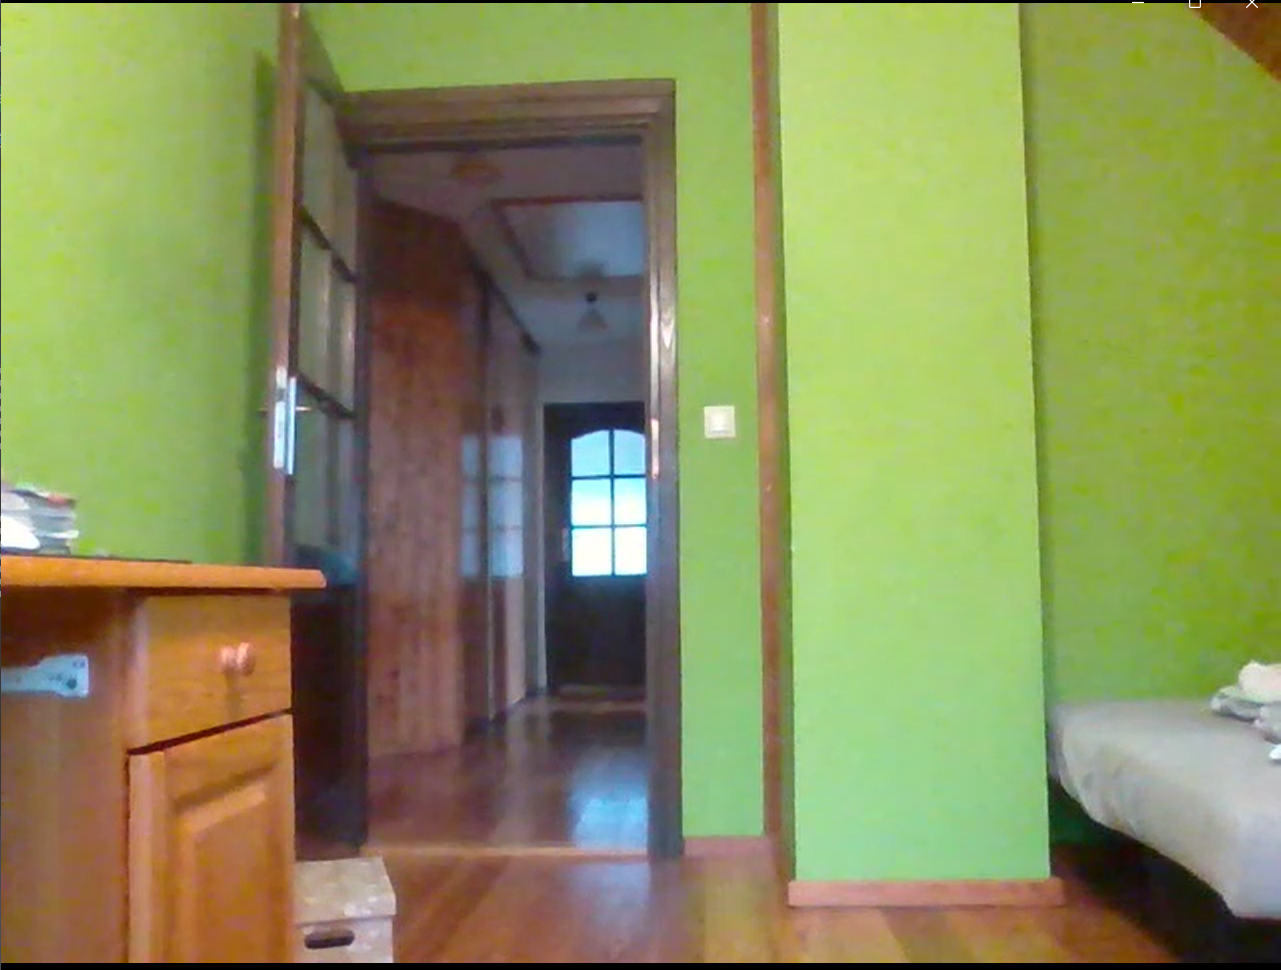
\includegraphics[width=\linewidth]{r_test_dokładności/vid_pics/1_1.png}
    \caption{Pomieszczenie, w którym nagrano filmy.}
    \label{fig:test-dokladnosc-scena}
\end{figure}

\begin{figure}[H]
    \centering
    \begin{minipage}{0.32\textwidth}
        \centering
        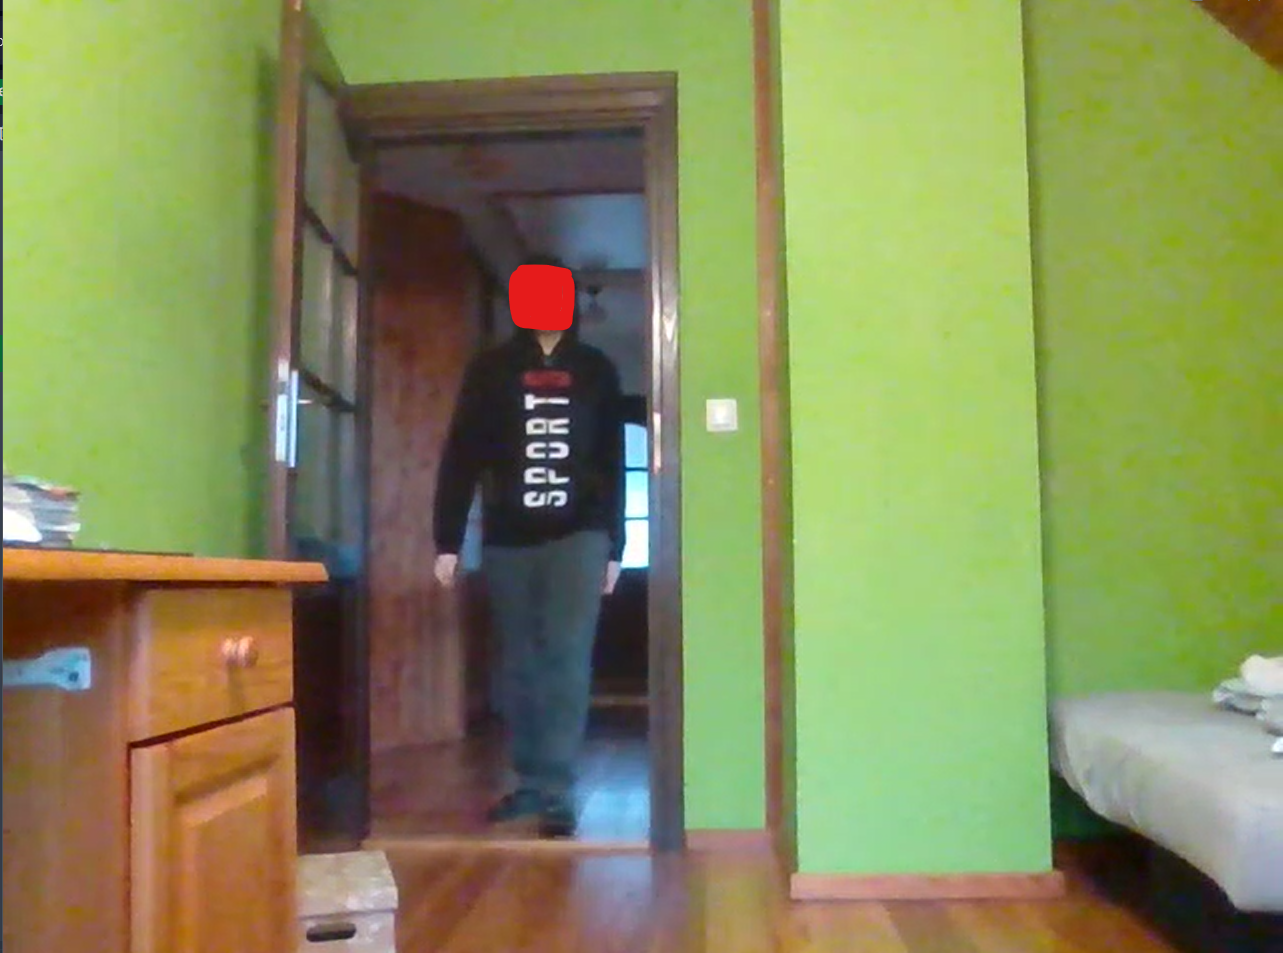
\includegraphics[width=\linewidth]{r_test_dokładności/vid_pics/1_2.png}
        \caption{Klatka filmu z człowiekiem.}
    \end{minipage}\hfill
    \begin{minipage}{0.32\textwidth}
        \centering
        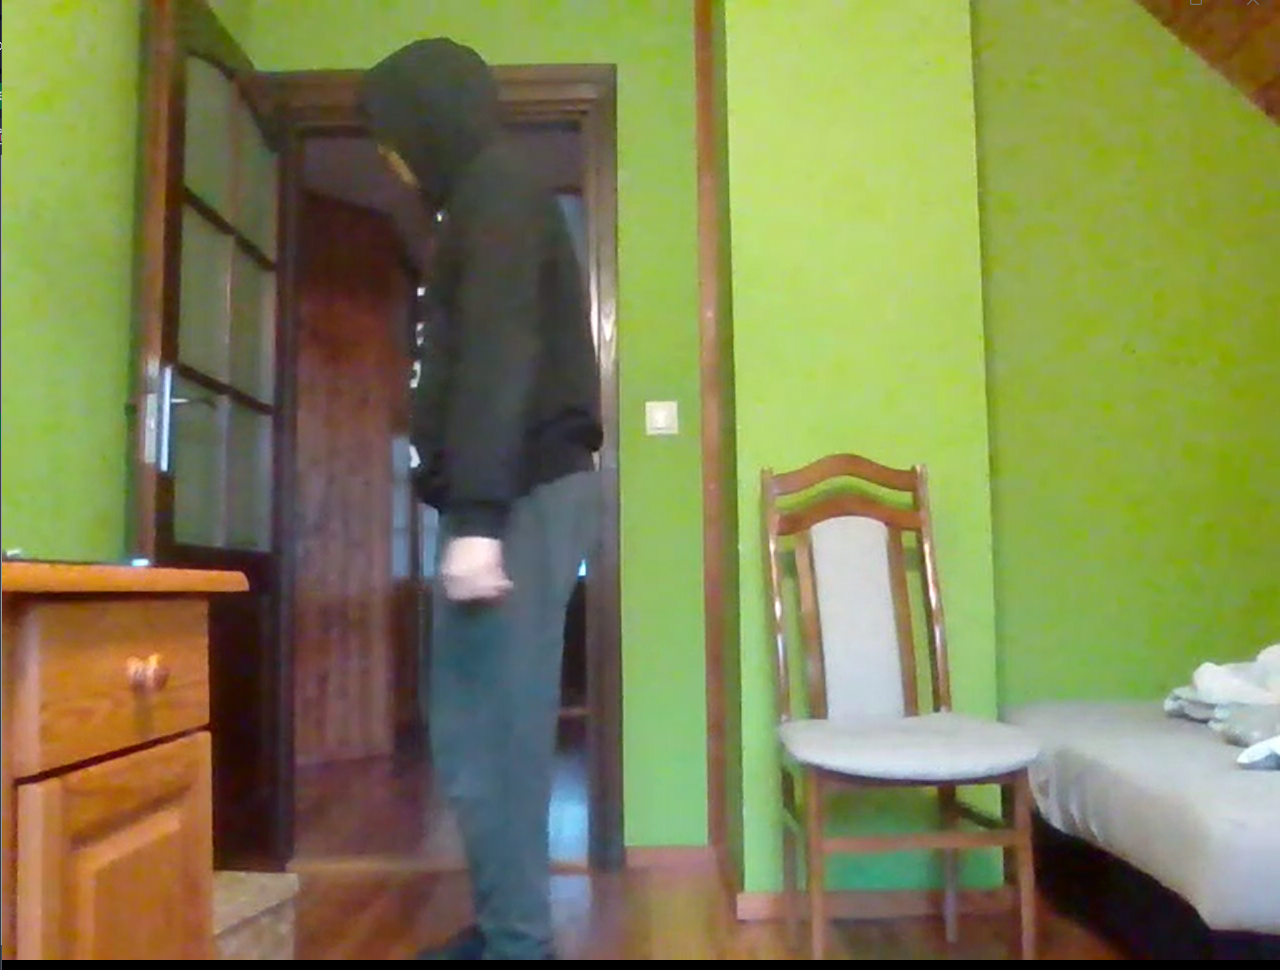
\includegraphics[width=\linewidth]{r_test_dokładności/vid_pics/1c_2.png}
        \caption{Klatka filmu z człowiekiem i krzesłem.}
    \end{minipage}\hfill
    \begin{minipage}{0.32\textwidth}
        \centering
        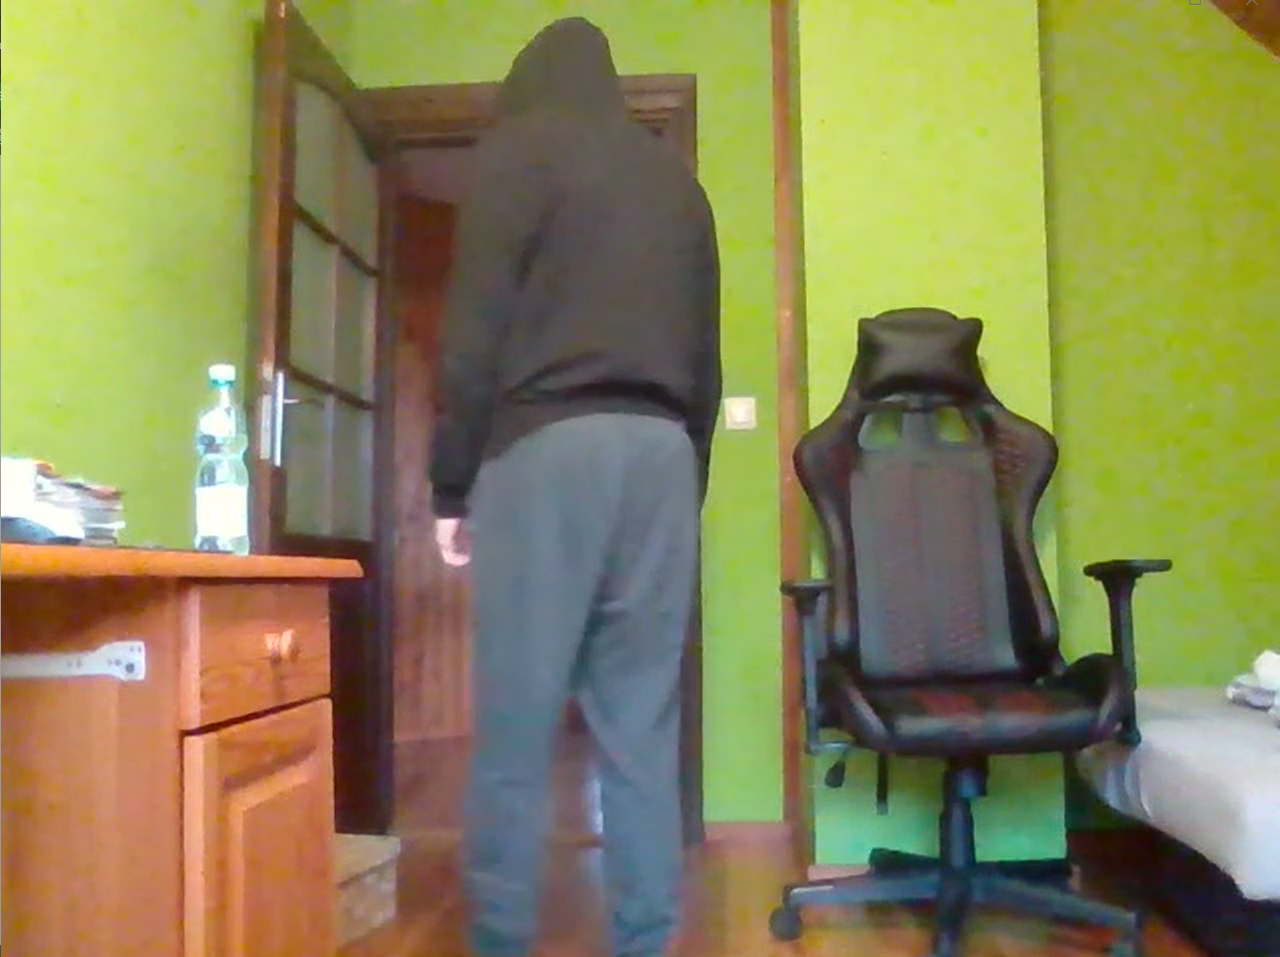
\includegraphics[width=\linewidth]{r_test_dokładności/vid_pics/1g_2.png}
        \caption{Klatka filmu z człowiekiem i fotelem.}
    \end{minipage}
    \caption{Prezentacja użytych obiektów.}
    \label{fig:all_objects}
\end{figure}
Filmy można podzielić na trzy kategorie ze względu na różne obecne w nim obiekty (wizualizacja objektów: rysunek \ref{fig:all_objects}):
\begin{itemize}
    \item człowiek
    \item człowiek, krzesło
    \item człowiek, fotel dla graczy (dalej nazywanym fotelem)
\end{itemize}
Krzesło oraz fotel to obiekty, z perspektywy filmów, statyczne --- przez całą długość filmu, na których występują, są one umieszczone w jednej lokalizacji, a inne obiekty nie mają z nimi fizycznej integracji.
Natomiast człowiek jest obiektem ruchomym. Jest on nieobecny przez pierwszą część każdego filmu. W drugiej części przechodzi on przez próg pomieszczenia, przybliża się do pewnego punktu w obiektywie i na koniec filmu robi jeden pełen obrót w okół własnej osi. 

Należy podkreślić ważne kwestie dotyczące nagranych filmów:
\begin{itemize}
    \item Obecne obiekty nie wchodzą ze sobą w integrację --- człowiek podczas ruchu, nie zasłania konturów krzesła oraz fotela.
    \item Generacja danych do testów nie odbywała się na każdej klatcę nagranego filmu. Użyto tylko klatek przedstawiających pełny kontur obiektów. Pełny kontur pojawia się w momencie przekroczenia progu wejścia do pomieszczenia. Użyto więc dwóch sekcji każdego filmu:
    \begin{itemize}
        \item Sekcja gdy człowiek był całkowicie nieobecny.
        \item Sekcja od moment przekroczenia progu.
    \end{itemize}
\end{itemize}

Dla każdej kategorii filmu nagrano cztery warianty z różnym poziomem oświetlenia w pomieszczeniu, co daje łącznie dwanaście plików wideo do analizy. Wizualne różnice między poziomami przedstawiono na rysunku \ref{fig:person_grid} (człowiek), rysunku \ref{fig:chair_grid} (człowiek, krzesło) i rysunku \ref{fig:game_grid} (człowiek, fotel). 
Dla każdego filmu, korzystając z modelu przestrzeni barw HSV, obliczono średnią jasność oraz saturacje filmu. Wartości te zaprezentowano w tabeli \ref{tab:saturation-value-table}. Obliczenia przeprowadzono poprzez wyznaczenie średniej wartości jasności oraz saturacji dla każdej klatki obrazu na podstawie wszystkich pikseli, a następnie wyznaczając średnią z uzyskanych wartości dla wszystkich klatek w filmie.
\begin{table}[H]
    \centering
    \caption{Jasność i nasycenie dla każdego nagranego filmu.}
    \begin{tabular}{|c|c|c|c|}
    \hline
    Nr sceny:          & Obecne obiekty    & Jasność & Nasycenie \\ \hline
    \multirow{3}{*}{1} & człowiek          & 152.73  & 107.3     \\ \cline{2-4} 
                       & człowiek, krzesło & 149.92  & 119.07    \\ \cline{2-4} 
                       & człowiek, fotel   & 152.68  & 111.47    \\ \hline
    \multirow{3}{*}{2} & człowiek          & 134.64  & 93.48     \\ \cline{2-4} 
                       & człowiek, krzesło & 139.14  & 90.71     \\ \cline{2-4} 
                       & człowiek, fotel   & 133.77  & 83.29     \\ \hline
    \multirow{3}{*}{3} & człowiek          & 41.59   & 123.48    \\ \cline{2-4} 
                       & człowiek, krzesło & 38.91   & 132.31    \\ \cline{2-4} 
                       & człowiek, fotel   & 38.12   & 124.31    \\ \hline
    \multirow{3}{*}{4} & człowiek          & 25.47   & 90.92     \\ \cline{2-4} 
                       & człowiek, krzesło & 25.3    & 100.8     \\ \cline{2-4} 
                       & człowiek, fotel   & 24.88   & 108.5     \\ \hline
    \end{tabular}
    \label{tab:saturation-value-table}
    \end{table}
\begin{figure}[H]
    \centering
    \begin{minipage}{0.45\textwidth}
        \centering
        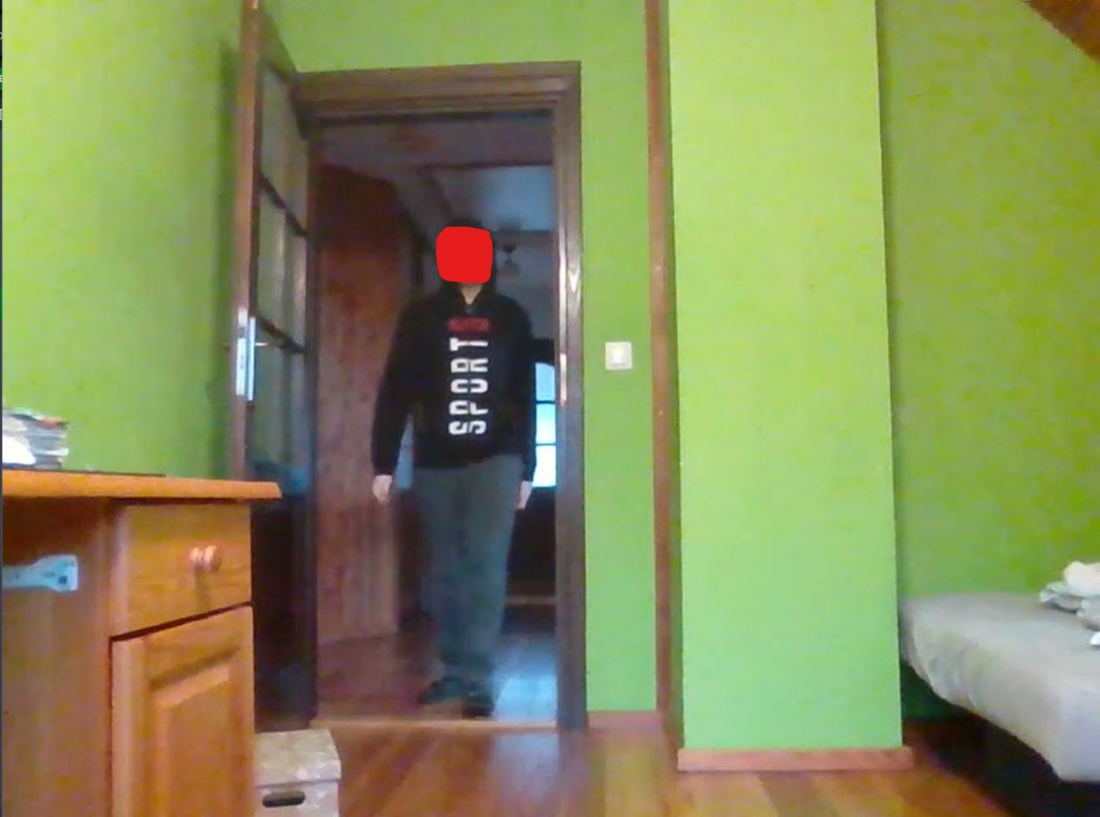
\includegraphics[width=\linewidth]{r_test_dokładności/vid_pics/1_2.jpg}
    \end{minipage}\hfill
    \begin{minipage}{0.45\textwidth}
        \centering
        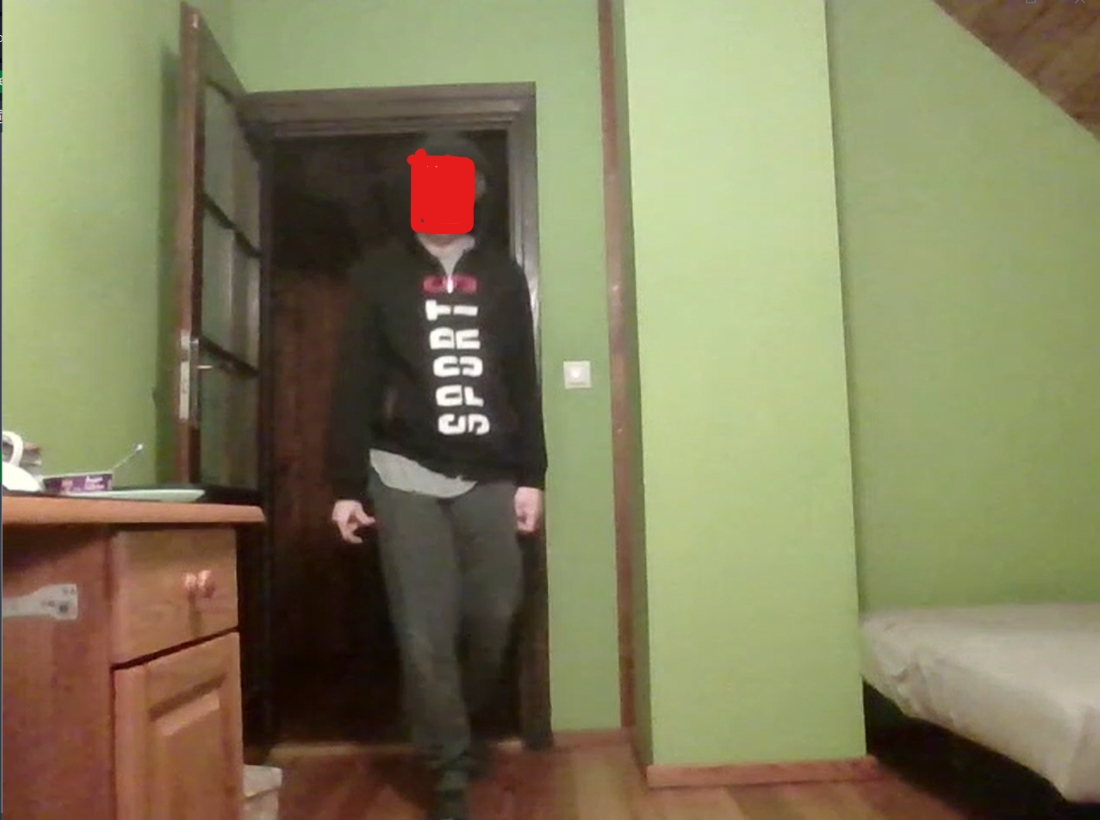
\includegraphics[width=\linewidth]{r_test_dokładności/vid_pics/2_2.jpg}
    \end{minipage}
    \vskip\baselineskip
    \begin{minipage}{0.45\textwidth}
        \centering
        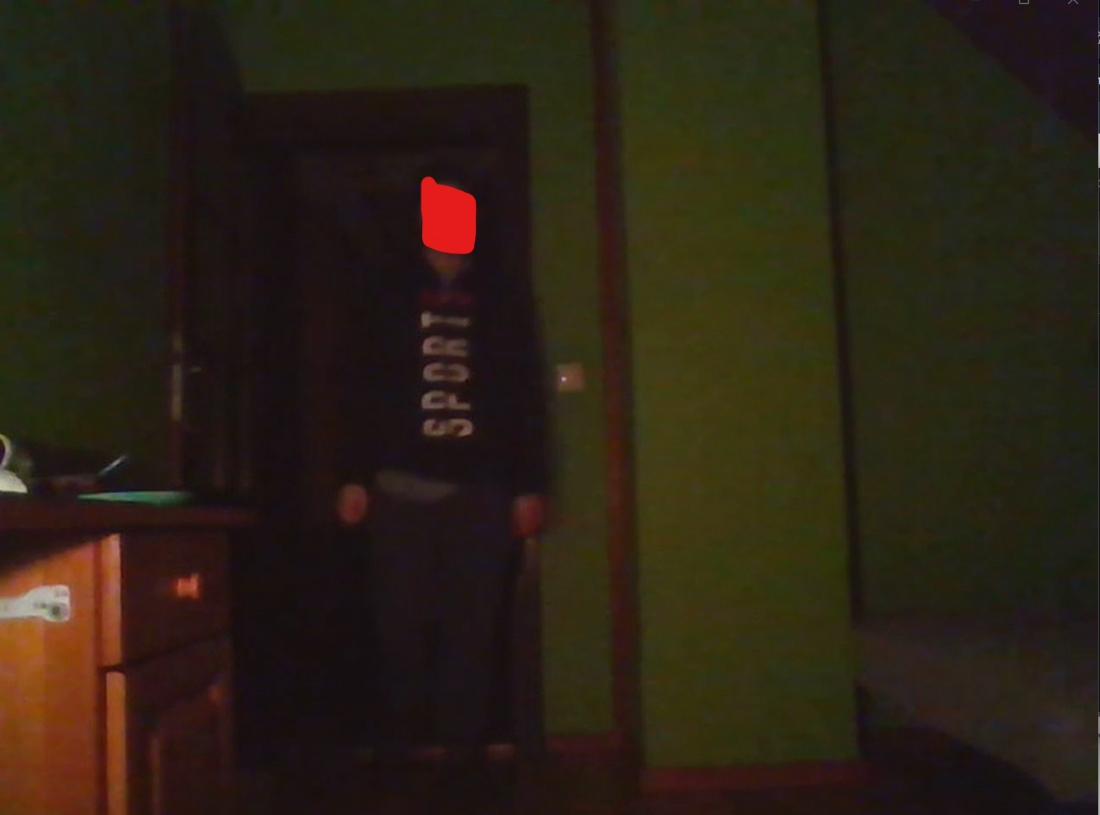
\includegraphics[width=\linewidth]{r_test_dokładności/vid_pics/3_2.jpg}
    \end{minipage}\hfill
    \begin{minipage}{0.45\textwidth}
        \centering
        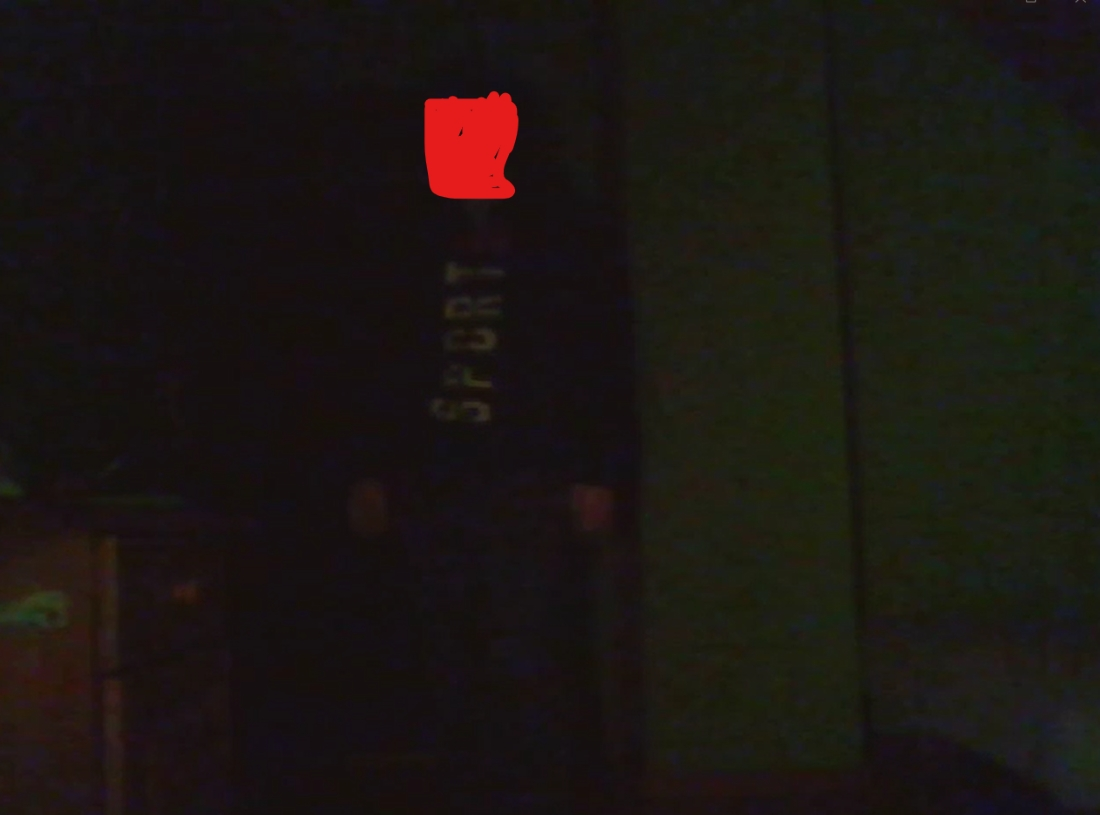
\includegraphics[width=\linewidth]{r_test_dokładności/vid_pics/4_2.jpg}
    \end{minipage}
    \caption{Poziomy oświetlenia dla filmów z obecnym człowiekiem}
    \label{fig:person_grid}
\end{figure}
\begin{figure}[H]
    \centering
    \begin{minipage}{0.45\textwidth}
        \centering
        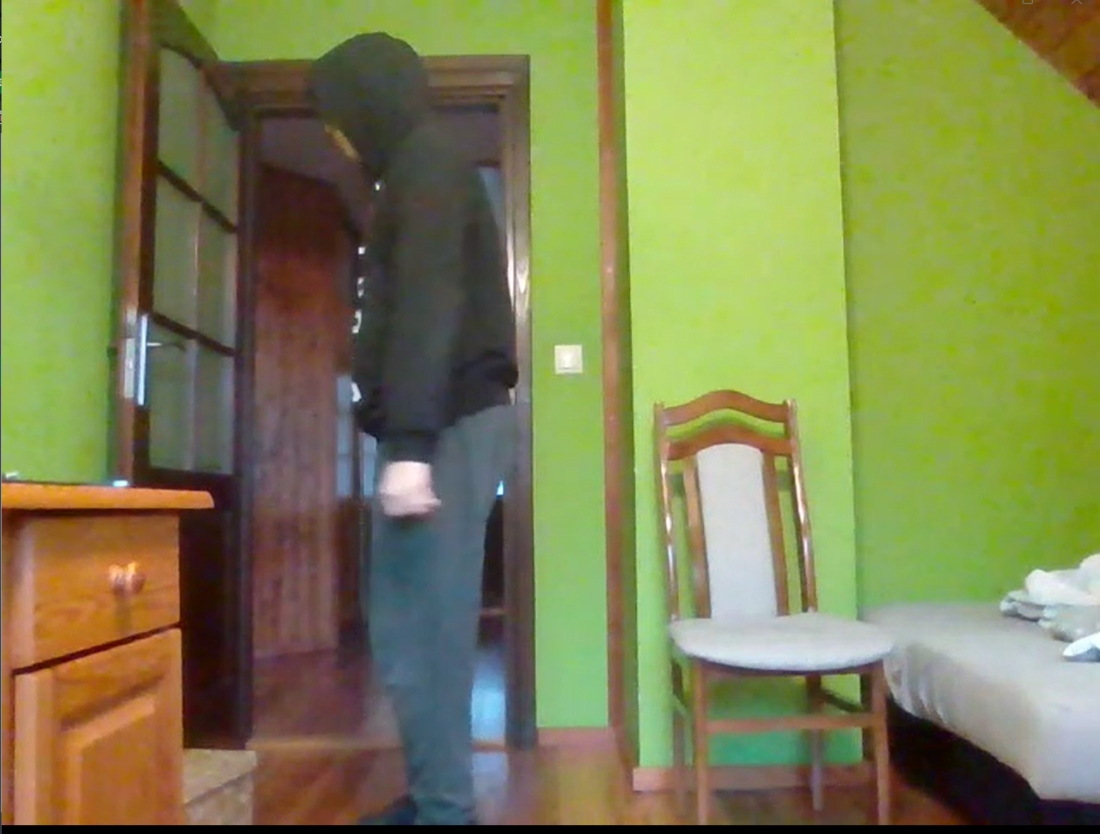
\includegraphics[width=\linewidth]{r_test_dokładności/vid_pics/1c_2.jpg}
    \end{minipage}\hfill
    \begin{minipage}{0.45\textwidth}
        \centering
        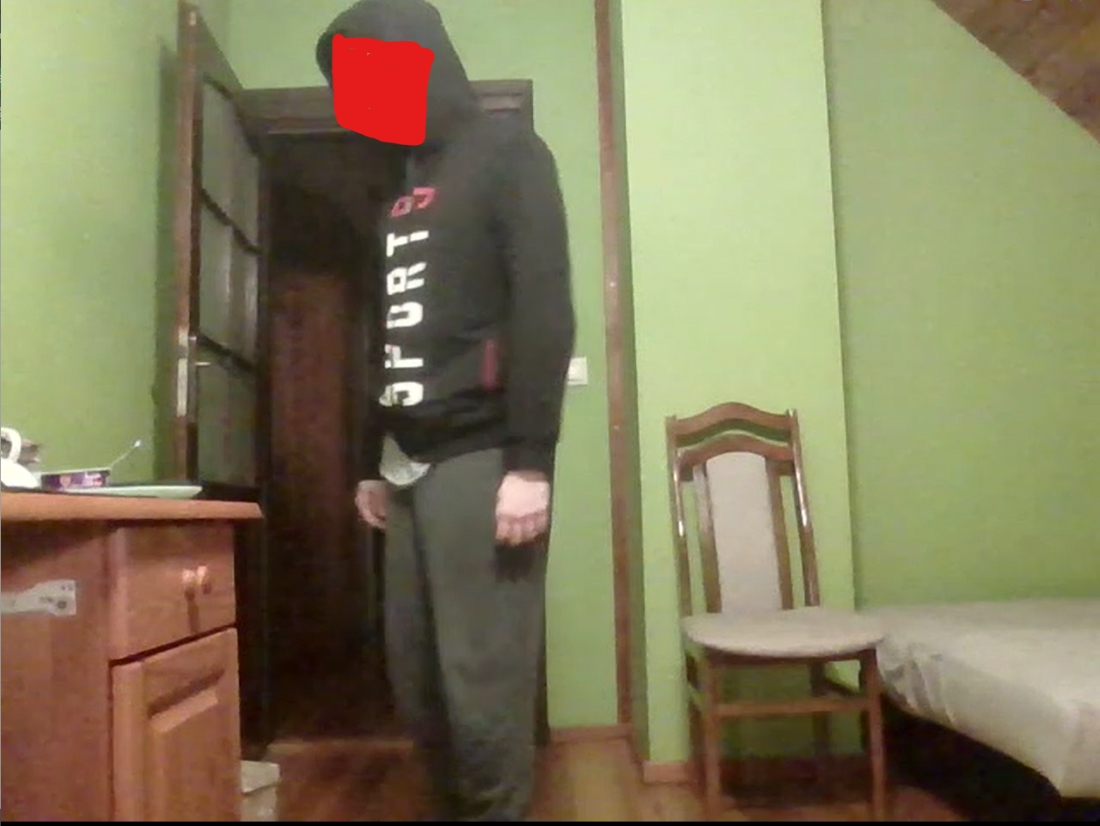
\includegraphics[width=\linewidth]{r_test_dokładności/vid_pics/2c_2.jpg}
    \end{minipage}
    \vskip\baselineskip
    \begin{minipage}{0.45\textwidth}
        \centering
        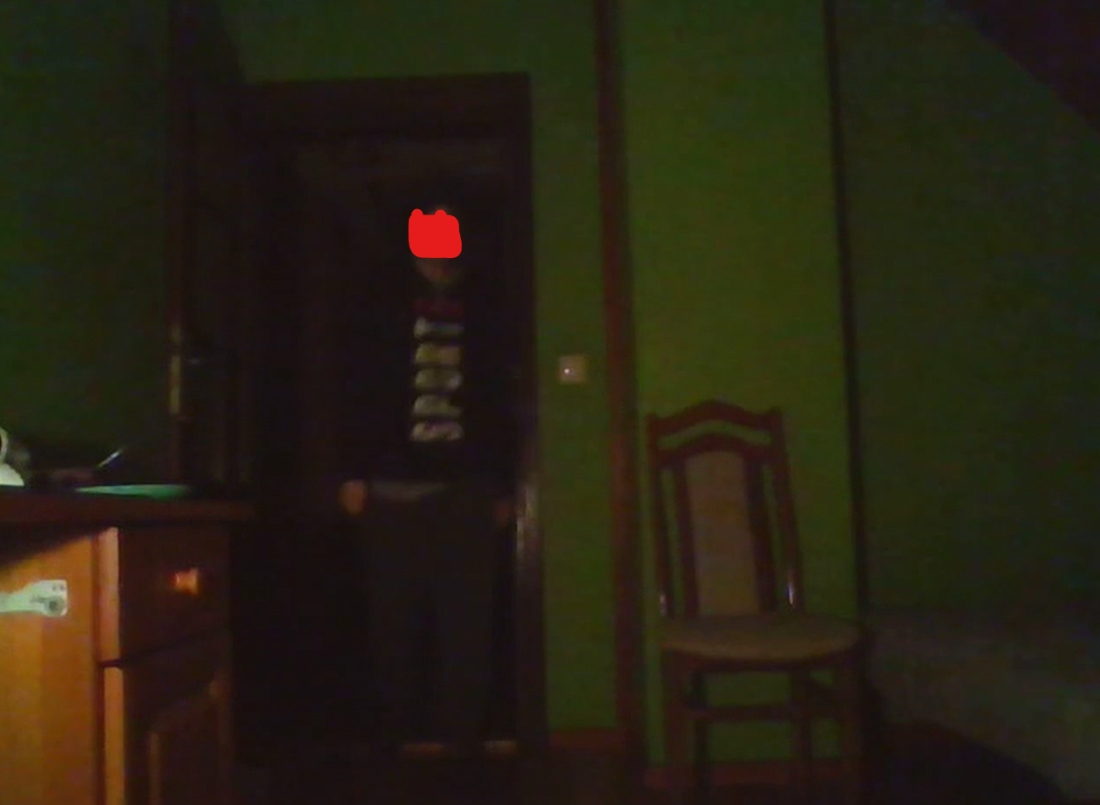
\includegraphics[width=\linewidth]{r_test_dokładności/vid_pics/3c_2.jpg}
    \end{minipage}\hfill
    \begin{minipage}{0.45\textwidth}
        \centering
        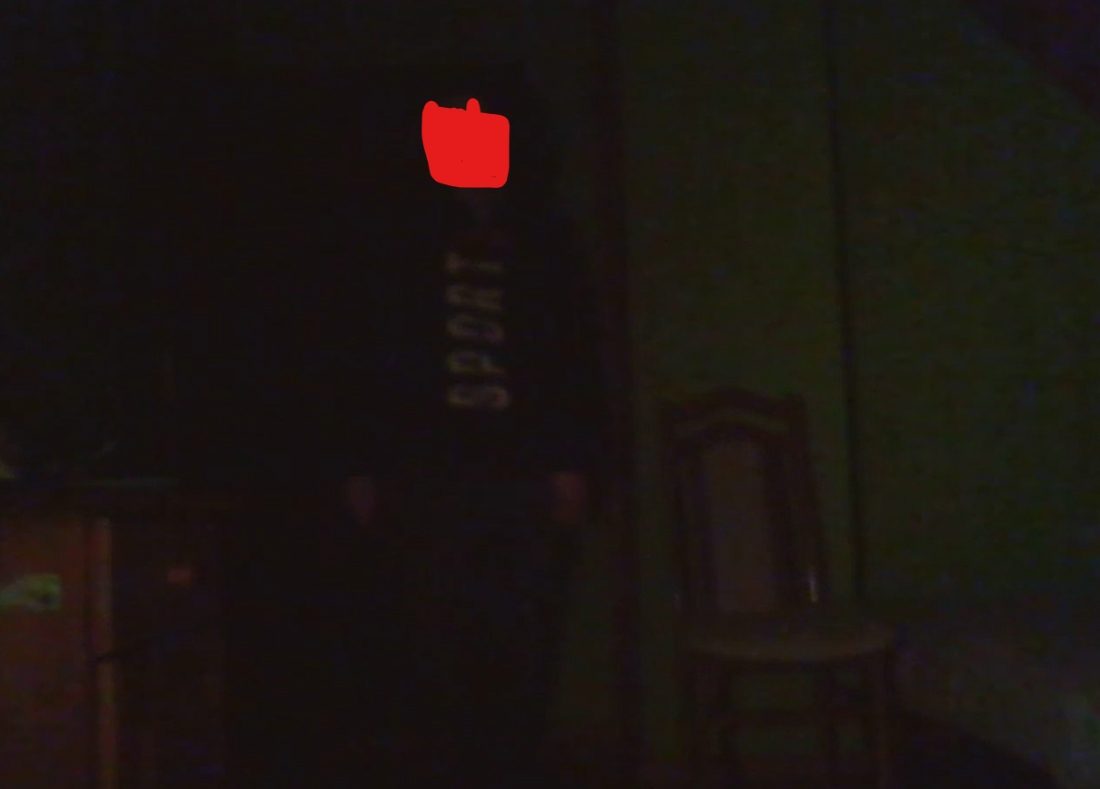
\includegraphics[width=\linewidth]{r_test_dokładności/vid_pics/4c_2.jpg}
    \end{minipage}
    \caption{Poziomy oświetlenia dla filmów z obecnym człowiekiem i krzesłem}
    \label{fig:chair_grid}
\end{figure}
\begin{figure}[H]
    \centering
    \begin{minipage}{0.45\textwidth}
        \centering
        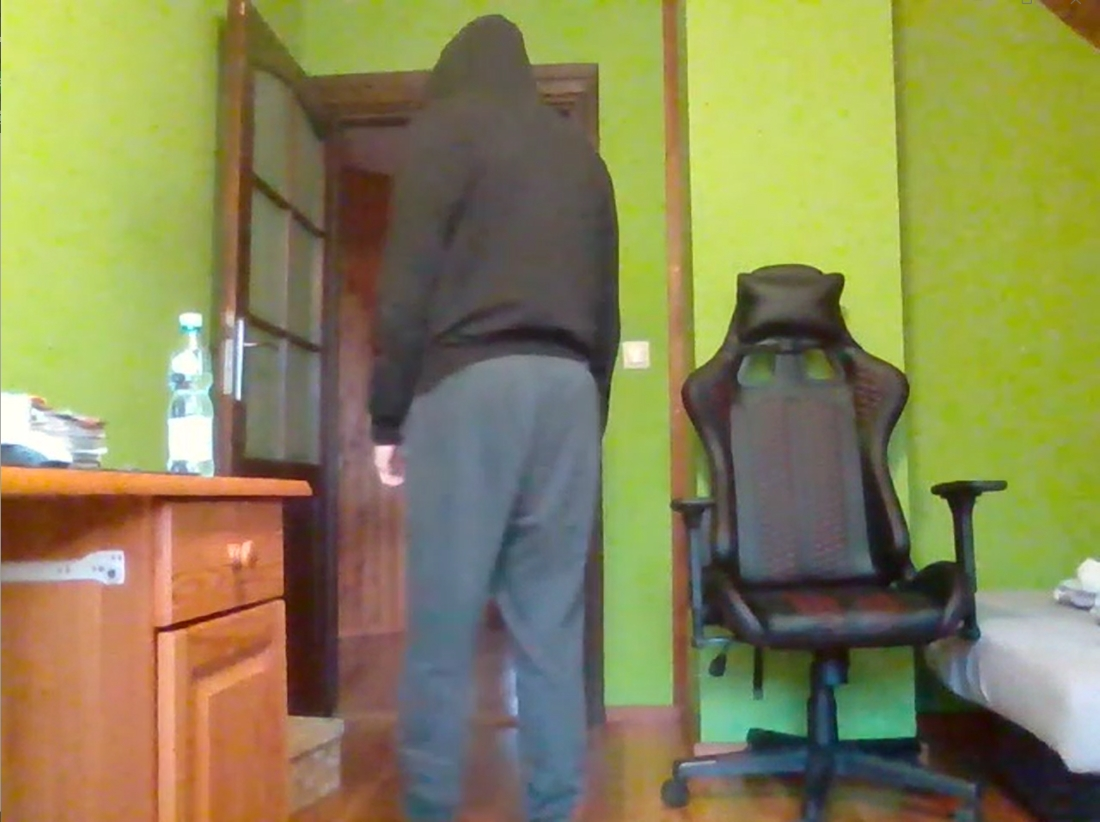
\includegraphics[width=\linewidth]{r_test_dokładności/vid_pics/1g_2.jpg}
    \end{minipage}\hfill
    \begin{minipage}{0.45\textwidth}
        \centering
        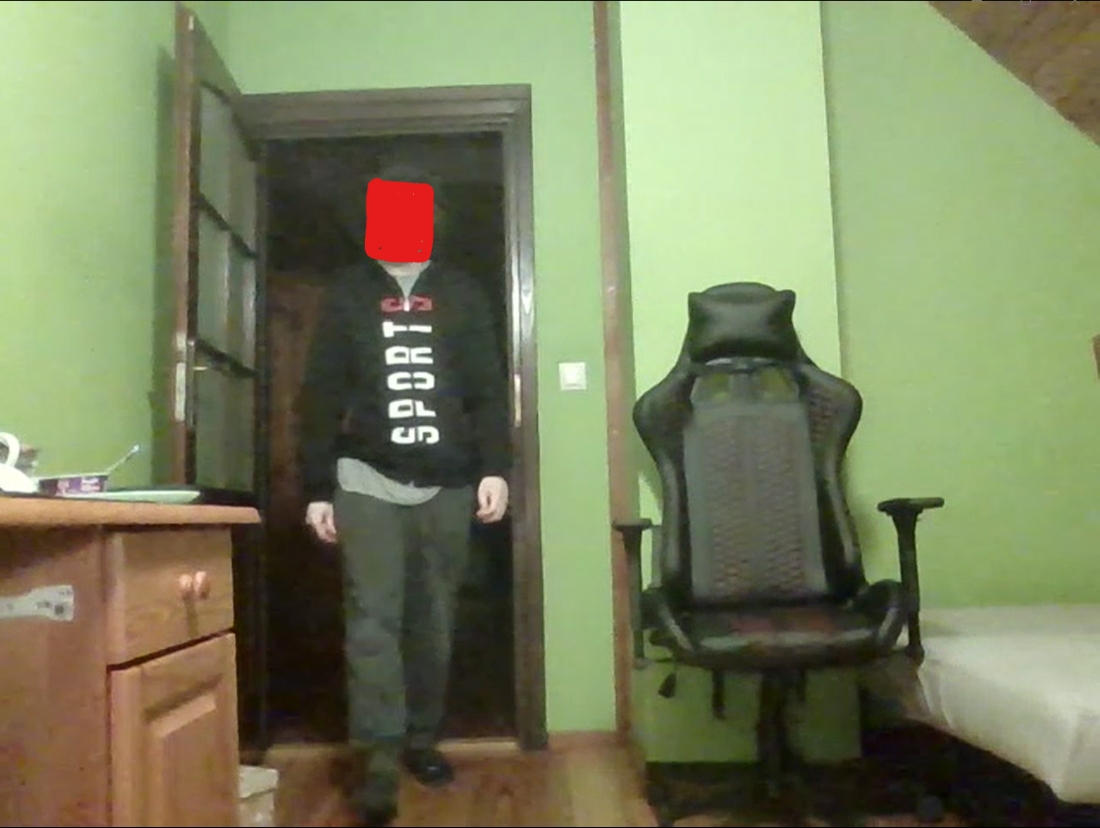
\includegraphics[width=\linewidth]{r_test_dokładności/vid_pics/2g_2.jpg}
    \end{minipage}
    \vskip\baselineskip
    \begin{minipage}{0.45\textwidth}
        \centering
        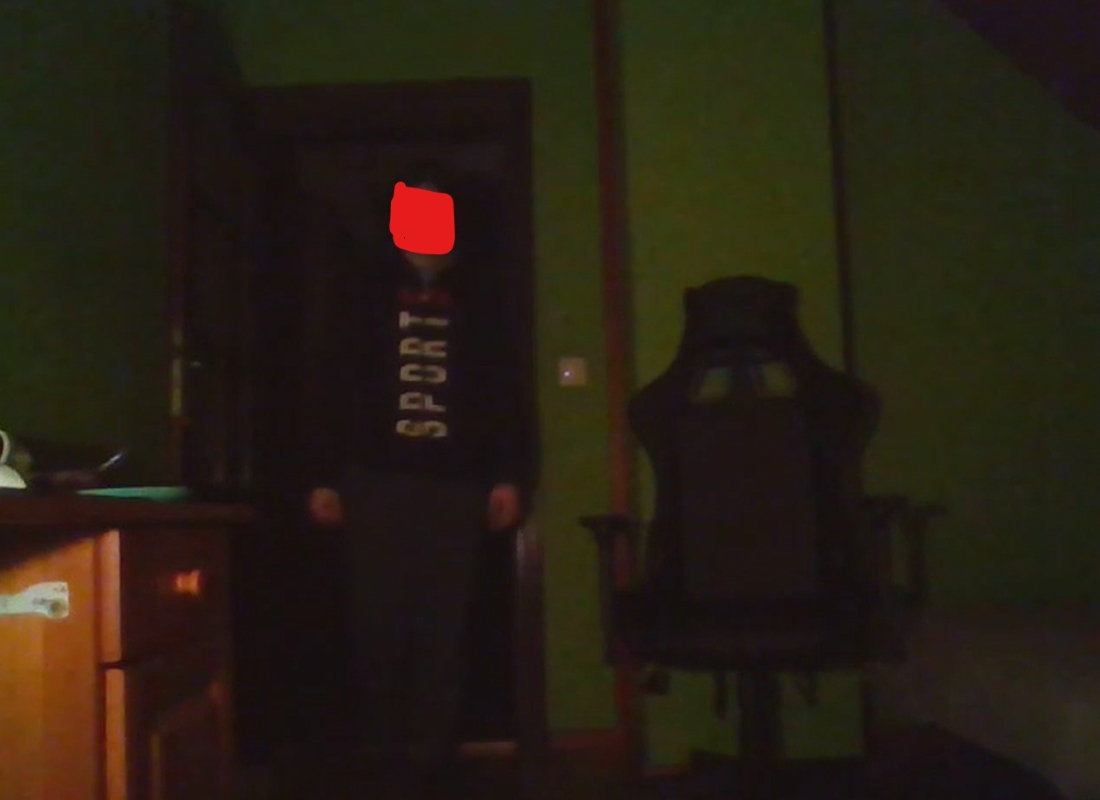
\includegraphics[width=\linewidth]{r_test_dokładności/vid_pics/3g_2.jpg}
    \end{minipage}\hfill
    \begin{minipage}{0.45\textwidth}
        \centering
        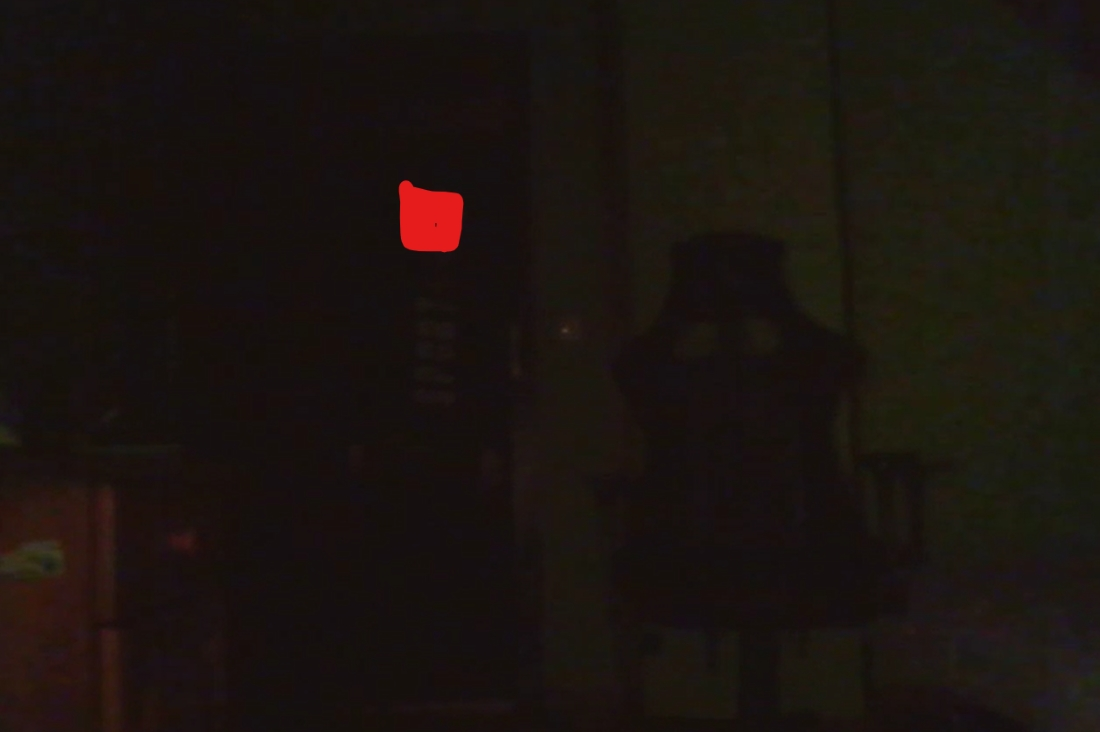
\includegraphics[width=\linewidth]{r_test_dokładności/vid_pics/4g_2.jpg}
    \end{minipage}
    \caption{Poziomy oświetlenia dla filmów z obecnym człowiekiem i fotelem}
    \label{fig:game_grid}
\end{figure}







\subsection{MEtryki}
Na podstawie opisanych dwunastu plików wideo wygenerowano dane do analizy w testach dla każdego z nich. Dane te to podstawowe metryki używane w klasyfikacji binarnej. Są to: wynik prawdziwy pozytywny (TP), wynik prawdziwy negatywny (TN), wynik fałszywy pozytywny (FP), Wynik fałszywy negatywny (FN). Zaprojektowane testy nie analizują klasyfikacji pod kątem całej sceny (wszystkich obecnych objektów), lecz indywidualnie dla każdej klasy obiektów. Biorąc to pod uwagę, definicję metryk skontruowano następująco: \\\\ \noindent
Znaczenie skrótów: \\
x -- pojedyńcze wystąpienie obiektu wykrywanej klasy \\
n*x -- wielokrotne wystąpienie obiektu wykrywanej klasy \\
$\emptyset$ -- brak wystąpienia obiektu wykrywanej klasy 
\begin{table}[H]
    \centering
    \caption{Definicja metryk generowanych podczas testów detekcji obiektów.}
    \begin{tabular}{|>{\centering\arraybackslash}m{2cm}|>{\centering\arraybackslash}m{2cm}|>{\centering\arraybackslash}m{2.5cm}|>{\raggedright\arraybackslash}m{7.5cm}|}
    \hline
    Metryka & Obiekty na nagraniu & Obiekty wykryte przez detektor & \multicolumn{1}{c|}{Opis} \\ \hline



    \multirow{2}{*}{TP} & \multirow{2}{*}{x} & x & \multirow{2}{7.5cm}{Detektor wykrył jeden lub więcej obiektów klasy x, gdy obiekt x był obecny.} \\ \cline{3-3}

     &  & n*x & \\ \cline{1-4}



    TN & $\emptyset$ & $\emptyset$ & Detektor nie wykrył ani jednego obiektu klasy x, gdy obiekt x był nieobecny. \\ \hline

    

    \multirow{2}{*}{TN} & \multirow{2}{*}{$\emptyset$} & x & \multirow{2}{7.5cm}{Detektor wykrył jeden lub więcej obiektów klasy x, mimo że obiekt był nieobecny.} \\ \cline{3-3}

     &  & n*x & \\ \cline{1-4}



    FN & x & $\emptyset$ & Detektor nie wykrył ani jednego obiektu klasy x, mimo że obiekt był obecny. \\ \hline
    \end{tabular}
\end{table}
adasdasdas

